\documentclass[a4paper, 11pt]{article}
\usepackage{comment} % enables the use of multi-line comments (\ifx \fi) 
\usepackage{fullpage} % changes the margin

\usepackage{tabu} % for nice arrays	
% For confusion matrix %
\usepackage{array}
\usepackage{multirow}

\newcommand\MyBox[2]{
  \fbox{\lower0.75cm
     \vbox to 1.7cm{\vfil
      \hbox to 1.7cm{\hfil\parbox{1.4cm}{#1\\#2}\hfil}
      \vfil}%
   }%
}
%%%%%%%%%%%%%%%%%%%%%%%%%
\usepackage{graphicx} % For img insert
\newcommand{\ts}{\textsuperscript} %For numering 1st 2nd
%% Greek Format %%
%\usepackage[cm-default]{fontspec}
%\setromanfont{FreeSerif}
%\setsansfont{FreeSans}
%\setmonofont{FreeMono}
\usepackage{xltxtra}
\usepackage{xgreek}
\setmainfont[Mapping=tex-text]{GFS Didot}
%%%%%%%%%%%%%%%%%%

\begin{document}
%Header-Make sure you update this information!!!!
\noindent
\large\textbf{Ανάλυση FPR} \hfill \textbf{Αθανάσιος Μητσέλος} \\
\normalsize ΣΗΜΜΥ \hfill Ημερομηνία Ανάθεσης: 06/12/16  \\
ΕΜΠ\hfill Τρέχουσα Ημερομηνία: 09/05/17 \\


\section*{Εισαγωγή}
Στην παρούσα αναφορά θα γίνει παρουσίαση και ανάλυση των καταναλωτών που εκλαμβάνονται από τον αλγόριθμο μερικώς επιβλεπόμενης μάθησης σαν ύποπτα δείγματα, ενώ στην πραγματικότητα οι μετρήσεις τους είναι άθικτες. Με την ανάλυση αυτών των συμπεριφορών καθίσταται ευκολότερος ο επανασχεδιασμός του αλγορίθμου για να μην ενοχοποιεί τέτοιου είδους καταναλωτές. Όπως γίνεται σαφές η ελαχιστοποίηση των λαθών είναι καίριας σημασίας ειδικά όταν το λάθος ενοχοποιεί κάποιο καταναλωτή. \\
Σε κάθε καταναλωτή έχουν εκχωρηθεί κάποια χαρακτηριστικά που δεν θα αναλυθούν σε αυτή την αναφορά. Τα χαρακτηριστικά είναι τα εξής:    
\begin{enumerate}
\item{\textit{Ετήσια μέση τιμή ημίωρου}} Βρίσκεται ο μέσος όρος ημίωρου κάθε μέρας και για όλες τις μέρες του έτους βρίσκεται ο ετήσιος μέσος όρος.
\item{\textit{Ετήσια τυπική απόκλιση ημίωρου}} Βρίσκεται η τυπική απόκλιση κάθε μέρας και για όλες τις μέρες του έτους βρίσκεται ο ετήσιος μέσος όρος της τυπικής απόκλισης.
\item{\textit{Κινούμενος μέσος όρος μηνιαίου μέσου όρου}} Πρόκειται για υπό συνθήκη χαρακτηριστικό που αν παρατηρήσει κάποια σημαντική πτώση των καταναλώσεων τότε ψάχνει για την μέγιστη και την καταγράφει. 
\item{\textit{Κινούμενος μέσος όρος μηνιαίας τυπικής απόκλισης}} Πρόκειται για υπό συνθήκη χαρακτηριστικό που αν παρατηρήσει κάποια σημαντική πτώση της τυπικής απόκλισης τότε ψάχνει για την μέγιστη και την καταγράφει.
\item{\textit{Συμμετρική διαφορά καταναλώσεων}} Πρόκειται για υπό συνθήκη χαρακτηριστικό που παρατηρεί μια γενική συμπεριφορά όμοιων καταναλωτών ως προς τη χρονική στιγμή της ελάχιστης κατανάλωσης και ψάχνει για κάποια σημαντική πτώση της κατανάλωσης ανάμεσα σε 2 συμμετρικές χρονικές στιγμές με άξονα συμμετρίας την εκάστοτε χρονική στιγμή ελαχίστου.
\item{\textit{Συμμετρική διαφορά τυπικής απόκλισης}} Πρόκειται για υπό συνθήκη χαρακτηριστικό που παρατηρεί μια γενική συμπεριφορά όμοιων καταναλωτών ως προς τη χρονική στιγμή της ελάχιστης κατανάλωσης και ψάχνει για κάποια σημαντική πτώση της τυπικής απόκλισης ανάμεσα σε 2 συμμετρικές χρονικές στιγμές με άξονα συμμετρίας την εκάστοτε χρονική στιγμή ελαχίστου.
\item{\textit{Τμηματική διαφορά κατανάλωσης με όμοιους καταναλωτές}} Πρόκειται για υπό συνθήκη χαρακτηριστικό που παρατηρεί μια γενική συμπεριφορά όμοιων καταναλωτών ως προς τη χρονική στιγμή της ελάχιστης κατανάλωσης και ψάχνει για κάποια σημαντική πτώση της κατανάλωσης ανάμεσα στον καταναλωτή και τους όμοιούς του μετά την χρονική στιγμή της ελάχιστης κατανάλωσης.
\item{\textit{Τμηματική διαφορά τυπικής απόκλισης με όμοιους καταναλωτές}} Πρόκειται για υπό συνθήκη χαρακτηριστικό που παρατηρεί μια γενική συμπεριφορά όμοιων καταναλωτών ως προς τη χρονική στιγμή της ελάχιστης κατανάλωσης και ψάχνει για κάποια σημαντική πτώση της τυπικής απόκλισης ανάμεσα στον καταναλωτή και τους όμοιούς του μετά την χρονική στιγμή της ελάχιστης κατανάλωσης.
\end{enumerate}

\section*{Παράδειγμα 1}
\begin{figure}[ht!]
\centering
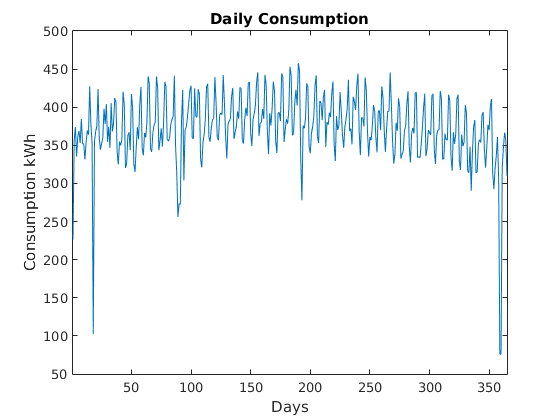
\includegraphics[width=100mm, height=70mm]{../../plots/FPR_analysis/Example_1.png}
\caption{Παράδειγμα 1\label{exFPR1}}
\end{figure}

\begin{center}
\begin{tabu} to 0.8\textwidth { | X[c] | X[c] | X[c] | X[c] | X[c] | X[c] | X[c] | X[c] |  }
 \hline
 \multicolumn{8}{|c|}{Χαρακτηριστικά 1ου Παραδείγματος} \\
 \hline
 1 & 2 & 3  & 4 & 5 & 6 & 7 & 8 \\
 \hline
15.55 &  14.48   &      0      &   0    &     0    &    0 & 132.5 & 0\\
\hline
\end{tabu}
\end{center}


\section*{Συνημμένα}
\ifx
Lab Notes, HelloWorld.ic, FooBar.ic,
\ref{exFPR1}.
\fi %comment me out

\begin{thebibliography}{9}
\ifx
\bibitem{Flueck}  Flueck, Alexander J. 2005. \emph{ECE 100}[online]. Chicago: Illinois Institute of Technology, Electrical and Computer Engineering Department, 2005 [cited 30
August 2005]. Available from World Wide Web: (http://www.ece.iit.edu/~flueck/ece100).
\fi
\end{thebibliography}

\end{document}
